\section{Experiments}

\begin{frame}<beamer>{Outline}
    \tableofcontents[currentsection,currentsubsection]
\end{frame}

\begin{frame}{MNIST dataset}

    \begin{itemize}
    \item 28x28 images of handwritten digits
    \item 50,000 training examples, 10,000 test examples, 10,000 validation examples
    \item Labels: 0 to 9 (one-hot encoding)
    \end{itemize}
    
    \begin{figure}[!tbp]
		\begin{center}
    	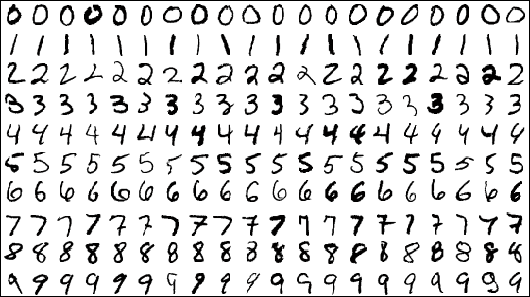
\includegraphics[width=2.4in]{mnist.png}
		\end{center}
	\end{figure}
    
\end{frame}
    
\begin{frame}{Experiments}

	\begin{itemize}
    \item{ \textbf{Network structures} }
		\begin{center}
		\begin{tabular}{ | l | c | c | c | }
		\hline
		& \cellcolor[gray]{0.85} \# Layers & \cellcolor[gray]{0.85} \# Nodes & \cellcolor[gray]{0.85} \# Num \\
		& \cellcolor[gray]{0.85} (In,\textbf{Hidden},Out) & \cellcolor[gray]{0.85} (In,\textbf{Hidden},Out) &\cellcolor[gray]{0.85} Params \\ \hline
		Network1 & 1,\textbf{1},1 & 784,\textbf{1024},10 & 800,000 \\ 
		\hline 
		Network2 & 1,\textbf{2},1 & 784,\textbf{1024,1024},10 & 1,860,000 \\
		\hline
		\end{tabular}
		\end{center}
	\end{itemize}
	
	\begin{itemize}
	\item Serial, Parallelize over examples (Pthreads, CUDA)
	\item Serial (BLAS), Parallelize matrix computations (BLAS)
	\item Serial (Keras:Theano), Parallel (Keras:Theano), GPU (Keras:Theano)
	\end{itemize}
	
	Analyze time per epoch, gigaflops for each implementation \\
	Analyze speedup from parallelization over serial counterparts

\end{frame}

